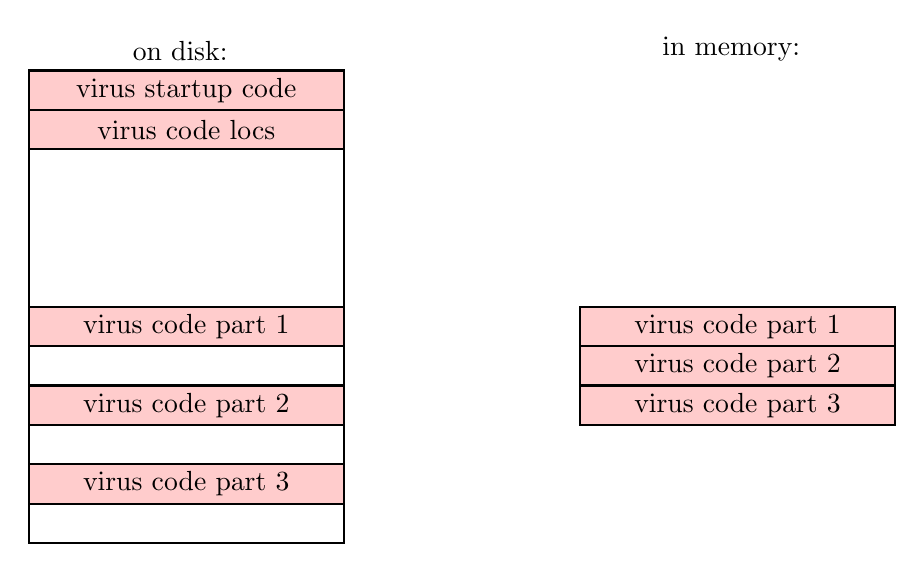
\begin{tikzpicture}
        \node[align=center,anchor=south] at (2, 0) { on disk: };
    \draw[fill=red!20,thick] (0, 0) rectangle (4, -0.5) node[midway] {virus startup code};
    \draw[fill=red!20,thick] (0, -0.5) rectangle (4, -1) node[midway] {virus code locs};
    \draw[thick] (0, -1) rectangle (4, -6);
    \draw[fill=red!20,thick] (0, -3) rectangle (4, -3.5)
        node[midway] {virus code part 1};
    \draw[fill=red!20,thick] (0, -4) rectangle (4, -4.5)
        node[midway] {virus code part 2};
    \draw[fill=red!20,thick] (0, -5) rectangle (4, -5.5)
        node[midway] {virus code part 3};
    \begin{scope}[xshift=7cm]
        \node[align=center,anchor=south] at (2, 0) { in memory: };
        \draw[fill=red!20,thick] (0, -3) rectangle (4, -3.5)
            node[midway] {virus code part 1};
        \draw[fill=red!20,thick] (0, -3.5) rectangle (4, -4)
            node[midway] {virus code part 2};
        \draw[fill=red!20,thick] (0, -4) rectangle (4, -4.5)
            node[midway] {virus code part 3};
    \end{scope}
    \end{tikzpicture}